\documentclass[tikz,border=12pt]{standalone}
\usepackage[T1]{fontenc}
\usepackage{mathpazo}
\usepackage{amsmath,amssymb}
\usetikzlibrary{arrows.meta, positioning, calc, fit, patterns, decorations.pathreplacing}

\definecolor{stblue}{HTML}{7B97AD}
\definecolor{rwgold}{HTML}{B8995E}
\definecolor{sage}{HTML}{7A9A7E}
\definecolor{dkbrown}{HTML}{3D3530}
\definecolor{wmgray}{HTML}{7B7067}
\definecolor{cream}{HTML}{F9F6F0}
\definecolor{border}{HTML}{D4C9B8}
\definecolor{terracotta}{HTML}{C47A6A}
\definecolor{lavender}{HTML}{907EA0}

\begin{document}
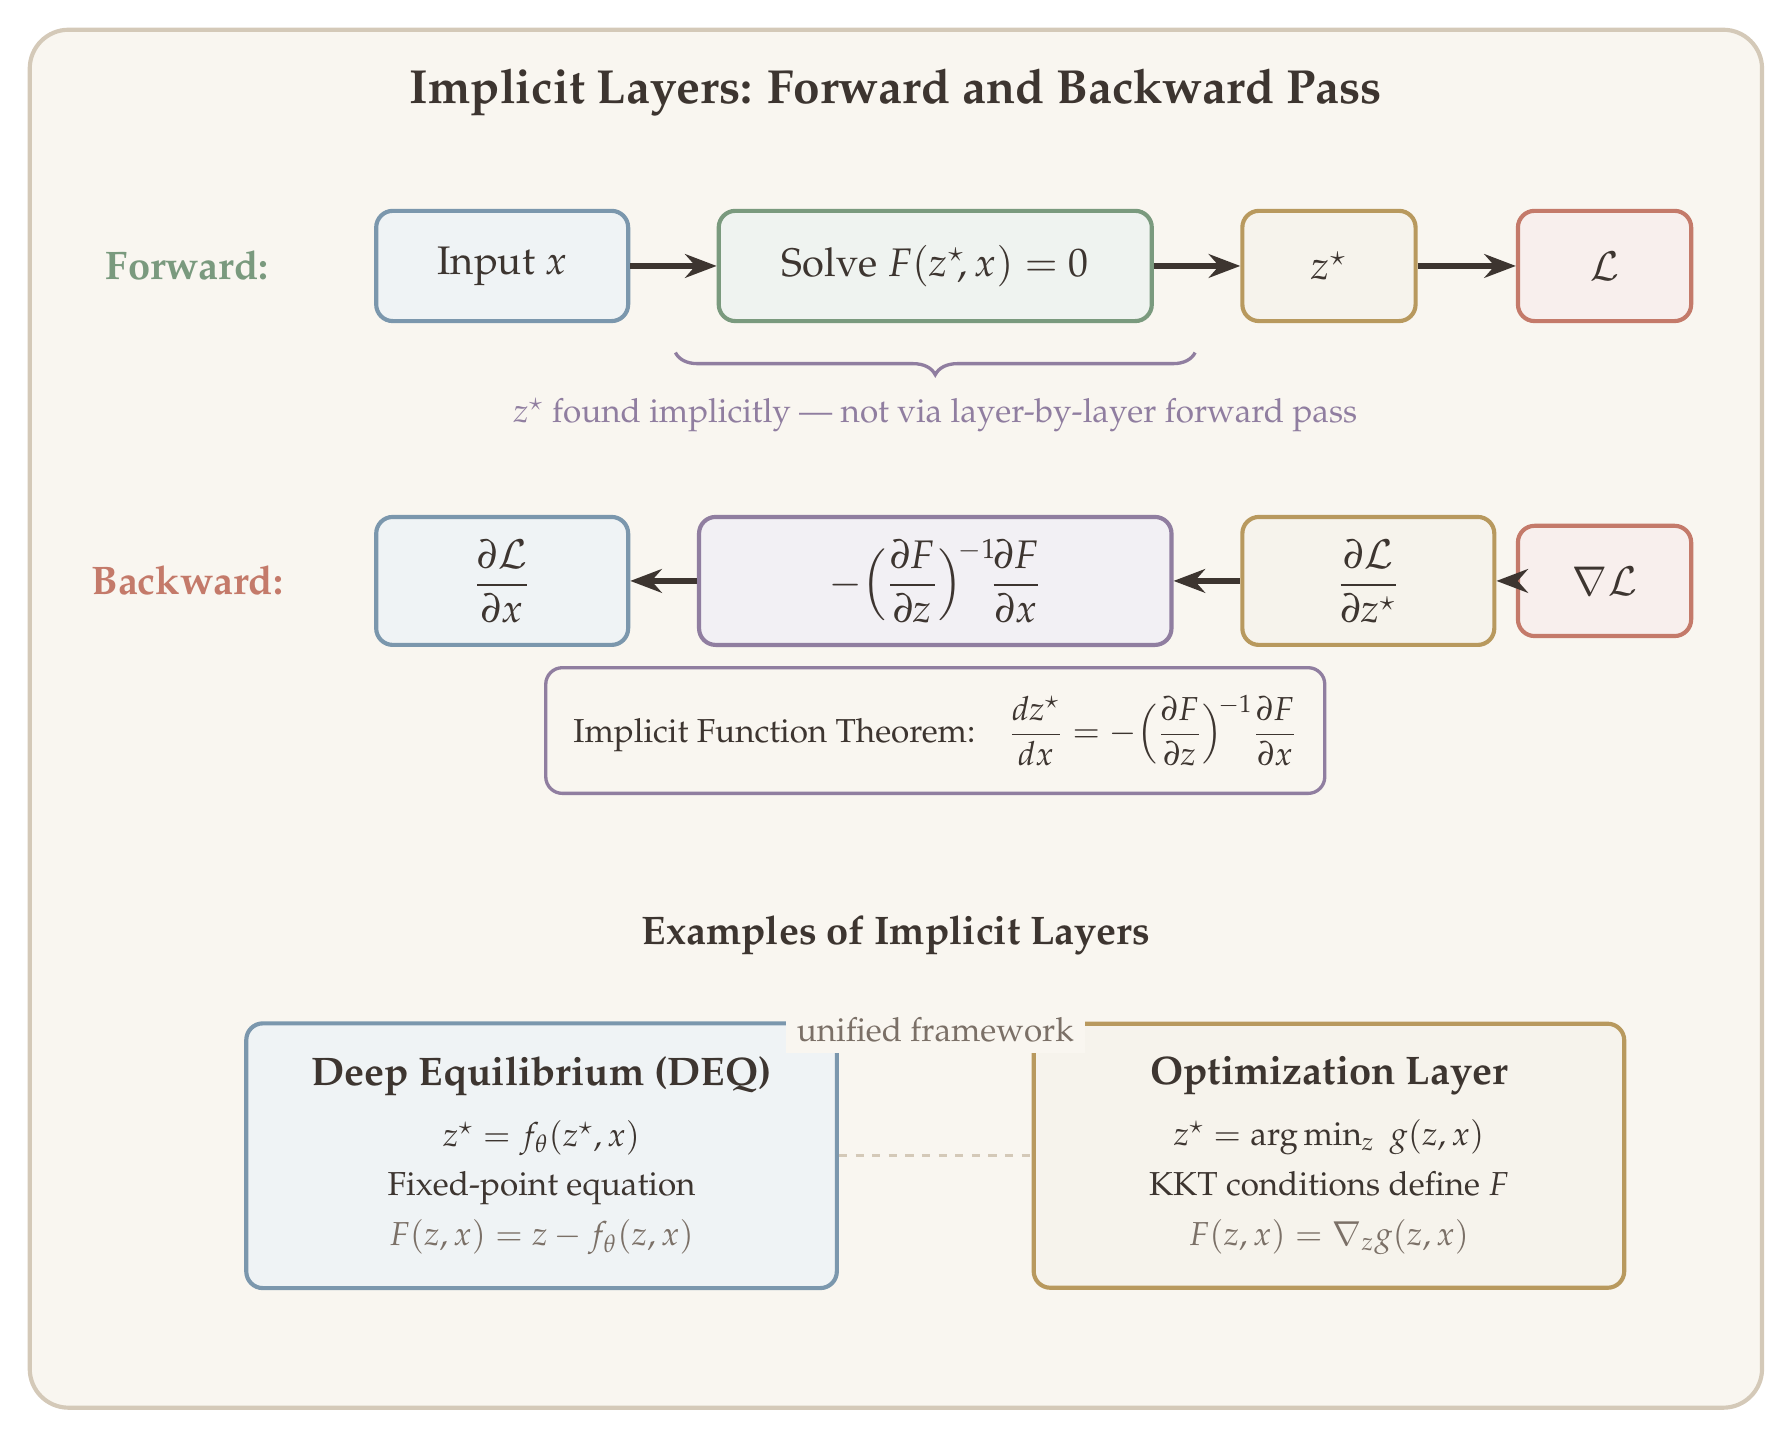
\begin{tikzpicture}[>={Stealth[length=4mm, width=3mm]}, line width=1.5pt,
  box/.style={fill=#1!12, draw=#1, line width=1.5pt, rounded corners=6pt,
              minimum height=1.4cm, minimum width=3.2cm, text=dkbrown, font=\Large,
              align=center, inner sep=8pt}]

% Background
\fill[cream, rounded corners=14pt] (-2,-8) rectangle (20,9.5);
\draw[border, line width=1.5pt, rounded corners=14pt] (-2,-8) rectangle (20,9.5);

% Title
\node[font=\LARGE\bfseries, text=dkbrown] at (9,8.7) {Implicit Layers: Forward and Backward Pass};

% =========== FORWARD PASS ===========
\node[font=\Large\bfseries, text=sage] at (0,6.5) {Forward:};

\node[box=stblue] (input) at (4,6.5) {Input $x$};
\node[box=sage, minimum width=5.5cm] (solver) at (9.5,6.5) {Solve $F(z^\star\!, x) = 0$};
\node[box=rwgold, minimum width=2.2cm] (zstar) at (14.5,6.5) {$z^\star$};
\node[box=terracotta, minimum width=2.2cm] (loss) at (18,6.5) {$\mathcal{L}$};

\draw[->, dkbrown, line width=2pt] (input) -- (solver);
\draw[->, dkbrown, line width=2pt] (solver) -- (zstar);
\draw[->, dkbrown, line width=2pt] (zstar) -- (loss);

% Brace annotation — mirror so bump points DOWN toward the label
\draw[decorate, decoration={brace, amplitude=8pt, mirror}, lavender, line width=1.2pt]
  (6.2,5.4) -- (12.8,5.4);
\node[font=\large, text=lavender] at (9.5,4.6)
  {$z^\star$ found implicitly --- not via layer-by-layer forward pass};

% =========== BACKWARD PASS ===========
\node[font=\Large\bfseries, text=terracotta] at (0,2.5) {Backward:};

\node[box=stblue] (grad_x) at (4,2.5) {$\dfrac{\partial \mathcal{L}}{\partial x}$};

\node[box=lavender, minimum width=6cm] (impl_diff) at (9.5,2.5)
  {$-\Bigl(\dfrac{\partial F}{\partial z}\Bigr)^{\!-1}\!\dfrac{\partial F}{\partial x}$};

\node[box=rwgold] (grad_z) at (15,2.5) {$\dfrac{\partial \mathcal{L}}{\partial z^\star}$};

% Backward arrows (reversed)
\draw[<-, dkbrown, line width=2pt] (grad_x) -- (impl_diff);
\draw[<-, dkbrown, line width=2pt] (impl_diff) -- (grad_z);

% nabla L label — separate to avoid overlap
\node[box=terracotta, minimum width=2.2cm] (nablaL) at (18,2.5) {$\nabla \mathcal{L}$};
\draw[<-, dkbrown, line width=2pt] (grad_z) -- (nablaL);

% IFT annotation
\node[fill=cream, draw=lavender, line width=1.2pt, rounded corners=6pt,
      font=\large, text=dkbrown, align=center, inner sep=10pt]
  at (9.5,0.6) {Implicit Function Theorem:\quad $\dfrac{dz^\star}{dx} = -\Bigl(\dfrac{\partial F}{\partial z}\Bigr)^{\!-1}\dfrac{\partial F}{\partial x}$};

% =========== EXAMPLES ===========
\node[font=\Large\bfseries, text=dkbrown] at (9,-2) {Examples of Implicit Layers};

% DEQ box
\node[fill=stblue!12, draw=stblue, line width=1.5pt, rounded corners=6pt,
      minimum height=2.8cm, minimum width=7.5cm, text=dkbrown, font=\large,
      align=center, inner sep=12pt] (deq) at (4.5,-4.8)
  {\textbf{\Large Deep Equilibrium (DEQ)}\\[8pt]
   $z^\star = f_\theta(z^\star, x)$\\[4pt]
   Fixed-point equation\\[4pt]
   {\color{wmgray}$F(z,x) = z - f_\theta(z,x)$}};

% OptLayer box
\node[fill=rwgold!12, draw=rwgold, line width=1.5pt, rounded corners=6pt,
      minimum height=2.8cm, minimum width=7.5cm, text=dkbrown, font=\large,
      align=center, inner sep=12pt] (optlayer) at (14.5,-4.8)
  {\textbf{\Large Optimization Layer}\\[8pt]
   $z^\star = \arg\min_z\; g(z, x)$\\[4pt]
   KKT conditions define $F$\\[4pt]
   {\color{wmgray}$F(z,x) = \nabla_z g(z,x)$}};

% Connecting line with label well above the boxes
\draw[border, line width=1pt, dashed] (deq.east) -- (optlayer.west);
\node[font=\large, text=wmgray, fill=cream, inner sep=4pt] at (9.5,-3.2) {unified framework};

\end{tikzpicture}
\end{document}
